
%% bare_jrnl_compsoc.tex
%% V1.4a
%% 2014/09/17
%% by Michael Shell
%% See:
%% http://www.michaelshell.org/
%% for current contact information.
%%
%% This is a skeleton file demonstrating the use of IEEEtran.cls
%% (requires IEEEtran.cls version 1.8a or later) with an IEEE
%% Computer Society journal paper.
%%
%% Support sites:
%% http://www.michaelshell.org/tex/ieeetran/
%% http://www.ctan.org/tex-archive/macros/latex/contrib/IEEEtran/
%% and
%% http://www.ieee.org/

%%*************************************************************************
%% Legal Notice:
%% This code is offered as-is without any warranty either expressed or
%% implied; without even the implied warranty of MERCHANTABILITY or
%% FITNESS FOR A PARTICULAR PURPOSE! 
%% User assumes all risk.
%% In no event shall IEEE or any contributor to this code be liable for
%% any damages or losses, including, but not limited to, incidental,
%% consequential, or any other damages, resulting from the use or misuse
%% of any information contained here.
%%
%% All comments are the opinions of their respective authors and are not
%% necessarily endorsed by the IEEE.
%%
%% This work is distributed under the LaTeX Project Public License (LPPL)
%% ( http://www.latex-project.org/ ) version 1.3, and may be freely used,
%% distributed and modified. A copy of the LPPL, version 1.3, is included
%% in the base LaTeX documentation of all distributions of LaTeX released
%% 2003/12/01 or later.
%% Retain all contribution notices and credits.
%% ** Modified files should be clearly indicated as such, including  **
%% ** renaming them and changing author support contact information. **
%%
%% File list of work: IEEEtran.cls, IEEEtran_HOWTO.pdf, bare_adv.tex,
%%                    bare_conf.tex, bare_jrnl.tex, bare_conf_compsoc.tex,
%%                    bare_jrnl_compsoc.tex, bare_jrnl_transmag.tex
%%*************************************************************************


% *** Authors should verify (and, if needed, correct) their LaTeX system  ***
% *** with the testflow diagnostic prior to trusting their LaTeX platform ***
% *** with production work. IEEE's font choices and paper sizes can       ***
% *** trigger bugs that do not appear when using other class files.       ***                          ***
% The testflow support page is at:
% http://www.michaelshell.org/tex/testflow/


\documentclass[10pt,conference,onecolumn,compsoc]{IEEEtran}


\usepackage{hyperref}
\usepackage{enumitem}
\setlist[itemize]{leftmargin=3 cm}
\setlist[enumerate]{leftmargin=3cm}



% *** CITATION PACKAGES ***
%
\ifCLASSOPTIONcompsoc
  % IEEE Computer Society needs nocompress option
  % requires cite.sty v4.0 or later (November 2003)
  \usepackage[nocompress]{cite}
\else
  % normal IEEE
  \usepackage{cite}
\fi
% cite.sty was written by Donald Arseneau
% V1.6 and later of IEEEtran pre-defines the format of the cite.sty package
% \cite{} output to follow that of IEEE. Loading the cite package will
% result in citation numbers being automatically sorted and properly
% "compressed/ranged". e.g., [1], [9], [2], [7], [5], [6] without using
% cite.sty will become [1], [2], [5]--[7], [9] using cite.sty. cite.sty's
% \cite will automatically add leading space, if needed. Use cite.sty's
% noadjust option (cite.sty V3.8 and later) if you want to turn this off
% such as if a citation ever needs to be enclosed in parenthesis.
% cite.sty is already installed on most LaTeX systems. Be sure and use
% version 5.0 (2009-03-20) and later if using hyperref.sty.
% The latest version can be obtained at:
% http://www.ctan.org/tex-archive/macros/latex/contrib/cite/
% The documentation is contained in the cite.sty file itself.



% *** GRAPHICS RELATED PACKAGES ***
%
\ifCLASSINFOpdf
   \usepackage[pdftex]{graphicx}
 
\else
 
\fi
% graphicx was written by David Carlisle and Sebastian Rahtz. It is
% required if you want graphics, photos, etc. graphicx.sty is already
% installed on most LaTeX systems. The latest version and documentation
% can be obtained at: 
% http://www.ctan.org/tex-archive/macros/latex/required/graphics/
% Another good source of documentation is "Using Imported Graphics in
% LaTeX2e" by Keith Reckdahl which can be found at:
% http://www.ctan.org/tex-archive/info/epslatex/
%
% latex, and pdflatex in dvi mode, support graphics in encapsulated
% postscript (.eps) format. pdflatex in pdf mode supports graphics
% in .pdf, .jpeg, .png and .mps (metapost) formats. Users should ensure
% that all non-photo figures use a vector format (.eps, .pdf, .mps) and
% not a bitmapped formats (.jpeg, .png). IEEE frowns on bitmapped formats
% which can result in "jaggedy"/blurry rendering of lines and letters as
% well as large increases in file sizes.
%
% You can find documentation about the pdfTeX application at:
% http://www.tug.org/applications/pdftex









% *** PDF, URL AND HYPERLINK PACKAGES ***
%
\usepackage{url}
% url.sty was written by Donald Arseneau. It provides better support for
% handling and breaking URLs. url.sty is already installed on most LaTeX
% systems. The latest version and documentation can be obtained at:
% http://www.ctan.org/tex-archive/macros/latex/contrib/url/
% Basically, \url{my_url_here}.




\begin{document}

\title{Maze Database\\ for UTM CSCI 352}
%
%

% received ..."  text while in non-compsoc journals this is reversed. Sigh.

\author{Grace Looney\\Matthew Pugh% <-this % stops a space
}

\IEEEtitleabstractindextext{%
\begin{abstract}
The goal of our project is to create a maze game using WPF applications and databases. We are planning for our game to be able to randomly cycle through at least five pregenerated mazes. Our target audience is gamers who enjoy solving puzzles and are looking for a short, fun diversion. Currently, we are still researching and planning out how to implement our project design.
\end{abstract}

}


% make the title area
\maketitle



\IEEEdisplaynontitleabstractindextext

\IEEEpeerreviewmaketitle



\section{Introduction}


For Maze, we are trying to accomplish a interactive WPF application that involves databases and computer generated mazes. We are using Eller's Algorithm to create the mazes due to its ability ro create infinite sized mazes very quickly. The mass of mazes will be stored as a 2d array in a database. The maze will be seen in an isometric view where the viewer will only be able to see a portion and the screen will move with the player. 

Maze is intended for people who enjoy puzzle games. It offers a simple distraction to the constant boredom most humans suffer from.  We hope our audience will achieve a sense of fullfiillment out of our game because they solved a maze or multiple mazes. 

\subsection{Background}
We want to our maze to be 'perfect' and  'orthogonal' \cite{Pullen}. A 'perfect' maze means that the maze lacks loops and closed cricuits. So the maze does not have any unreachable areas. In addition, 'perfect' implies that there is exactly one path. There are multiple ways to do this. For example, The best way to achieve this is to use to achieve an 'perfect' 'orthogonal' maze is to use Eller's Algorithm. Eller's Algorithm is incredibly fast and very memory efficient because it only requires storage proportional to only a single row. So in the future, we aim to get the application to make simple mazes on user-demand. 

We decided to do this project because it allows us to use databases and algorithms. Algorithms hold a special place in our hearts. They offer a way to implement something amazing efficiently. On the otherhand, databases are something new that we have learned in CSCI 352.


\subsection{Challenges}
We will most likely get stuck in implementing a database, Eller's algorithm, and the isometric view. We are both neophytes concerning databases, and we need to find a way so that we limit the amount of space that an array takes up. Eller's Algorithm requires implementers to understand sets and inner-relations of sets to arrays. The isometric view will require us to understand 3D graphics which none of us have experience in. 


\section{Scope}
Our project is done when we have a 'perfect' 'orthogonal' maze application with a view. It will be a functional application that calls on a database holding minimum of five mazes and be able to call on them at random. In addition, the user will be able to view a menu with buttons that'll allow it to randomly select a maze and format it to be viewed isometricly. 
\subsection{Stretch Goals:}
\begin{itemize}
\item Timed: The user can see how long it took them to complete that maze.
\item Scored: The user can earn points by collecting items across the maze.
\item Music: The user can have music while completing the maze.
\item Secret Buttons: The user can access special items or areas when standing on secret button

\end{itemize}


\subsection{Requirements}
As part of fleshing out the scope of your requirements, you'll also need to keep in mind both your functional and non-functional requirements.  These should be listed, and explained in detail as necessary.  Use this area to explain how you gathered these requirements.

\subsubsection{Functional}
\begin{itemize}
\item User needs to be able to interact with the maze
\item Application needs to be able to save 3 games
\item Application needs to be able to load any of the three saved games
\item Application will record high scores
\end{itemize}

\subsubsection{Non-Functional}
\begin{itemize}
\item Perfomance- Application will create mazes in a short amount of time
\item Scalability - Application will create mazes of differnent sizes
\end{itemize}

\subsection{Use Cases}
This subsection is arguably part of how you define your project scope (why it is in the Scope section...).  In a traditional Waterfall approach, as part of your requirements gathering phase (what does the product actually \emph{need} to do?), you will typically sit down with a user to develop use cases.

You should have a table listing all use cases discussed in the document, the ID is just the order it is listed in, the name should be indicative of what should happen, the primary actor is typically most important in an application where you may have different levels of users (think admin vs normal user), complexity is a best-guess on your part as to how hard it should be.  A lower number in priority indicates that it needs to happen sooner rather than later.  A sample table, or Use Case Index can be seen in Table \ref{tab:useCaseIndex}.




\begin{table}
\centering
\begin{tabular}{|c|c|c|c|c|}
\hline
Use Case ID & Use Case Name & Primary Actor & Complexity & Priority \\
\hline \hline
1 & Start New Game & Gamer & Med & 1\\
2 & Customize Maze & Gamer & Med & 2\\
3 & Save Game & Gamer & Med & 3\\
4 & Load Game & Gamer & Med  &3\\
5 & Calculate High Scores & Computer & Med & 3\\
6 & Play Game & Gamer & Hard & 1\\
7 & View Credits & Gamer & Easy & 4\\
\hline

\end{tabular}
\caption{Use case table}
\label{tab:useCaseIndex}
\end{table}


\begin{itemize}
\item[Use Case Number:] 1
\item[Use Case Name:] Start New Game 
\item[Description:] The gamer on our WPF application wants to play a new game. They will click the "New Game" Button, and this will start the off the Eller's algorithm to create a new maze. In addition, the maze will display after algorithm is completed. 
\item[Preconditons:]
\begin{itemize} 
\item Maze is downloaded
\item Maze has been opened
\end{itemize}

\item[Postconditons:]
\begin{itemize} 
\item New game will be started
\end{itemize}
\item[Invariants:]
\begin{itemize} 
\item New game function is working properly
\item Game runs as it is meant to
\end{itemize}
\end{itemize}


\begin{enumerate}
\item Select New Game from the main menu
\item Play game
\end{enumerate}

\begin{itemize}
\item[Use Case Number:] 2
\item[Use Case Name:] Customize Maze
\item[Description:] The gamer on our WPF application wants to edit their maze appearence or the sounds of the maze. The gamer clicks the "Settings" button. This will take the gamer to the settings menu, so they can customize the maze appearence.

\item[Preconditons:]
\begin{itemize} 
\item Maze is downloaded
\item Maze has been opened
\end{itemize}

\item[Postconditons:]
\begin{itemize} 
\item Current maze theme will be updated
\end{itemize}
\item[Invariants:]
\begin{itemize} 
\item Theme function is working properly
\item Music function is working properly
\item Customize function is working properly

\end{itemize}
\end{itemize}


\begin{enumerate}
\item Select settings from home screen
\item If desired theme already exists, then select it from the Theme menu
\item If desired theme does not exist, then move to the Customize menu
\item Select desired color for maze walls
\item Select desired color for maze floor
\item Select desired music setting from the Music menu
\item Save maze settings


\end{enumerate}
\begin{itemize}
\item[Use Case Number:] 3
\item[Use Case Name:] Save Game
\item[Description:] The gamer on our WPF application wants to save their unfinished maze. The gamer selects in the "save" button from the game view. They will be able to select one of the save spaces to save their maze to that memory spot.
\item[Preconditons:]
\begin{itemize} 
\item Maze is downloaded
\item Maze has been opened
\end{itemize}

\item[Postconditons:]
\begin{itemize} 
\item Current game is saved in desired save slot
\end{itemize}
\item[Invariants:]
\begin{itemize} 
\item Pause function is working properly
\item Save function is working properly
\end{itemize}
\end{itemize}


\begin{enumerate}
\item Click pause button
\item Click save button
\item Select a save slot
\item If save slot is currently being used, then decide whether or not to overwrite the previous save
\item Return to pause menu
\item End current game

\end{enumerate}

You will then need to continue to flesh out all use cases you have identified for your project.

\subsection{Interface Mockups}

\begin{figure}[ht!]
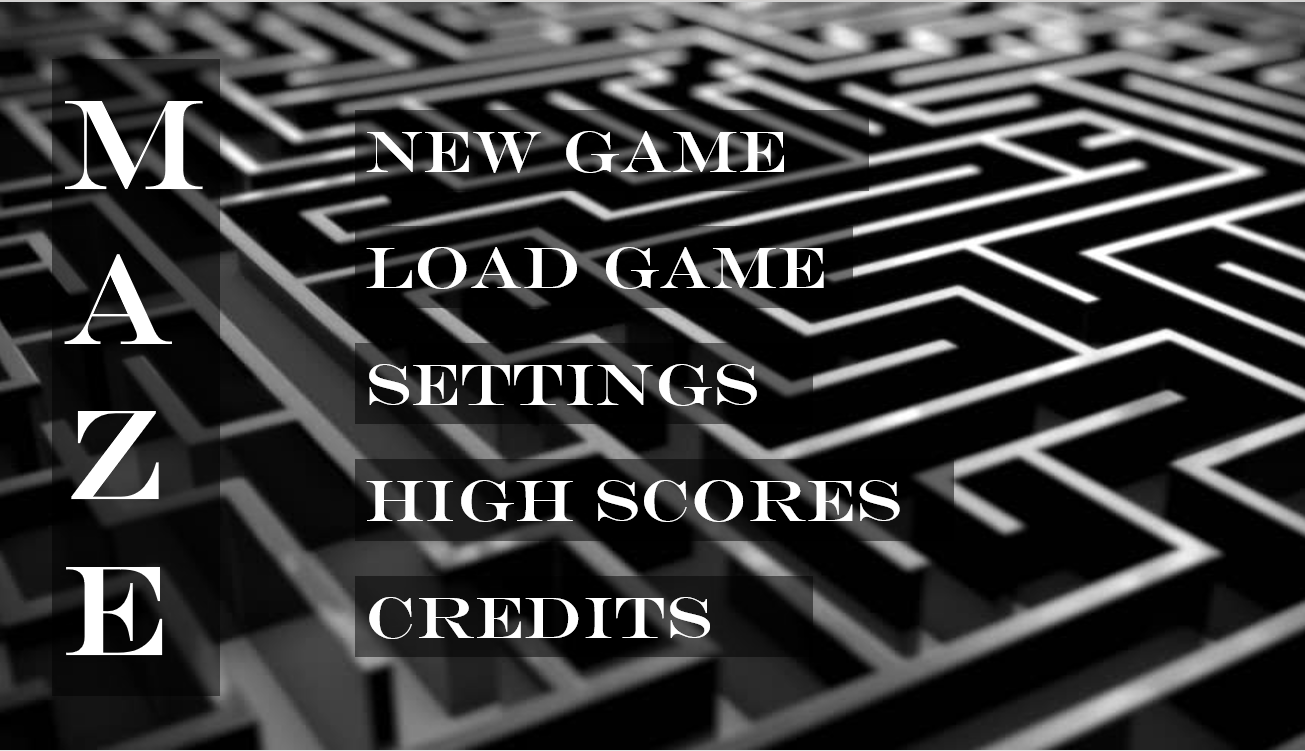
\includegraphics[height=150px, width=250px]{interface/Interface-Menu.png}
\caption{This is the Menu}
\label{Menu}
\end{figure}
\begin{figure}[ht!]
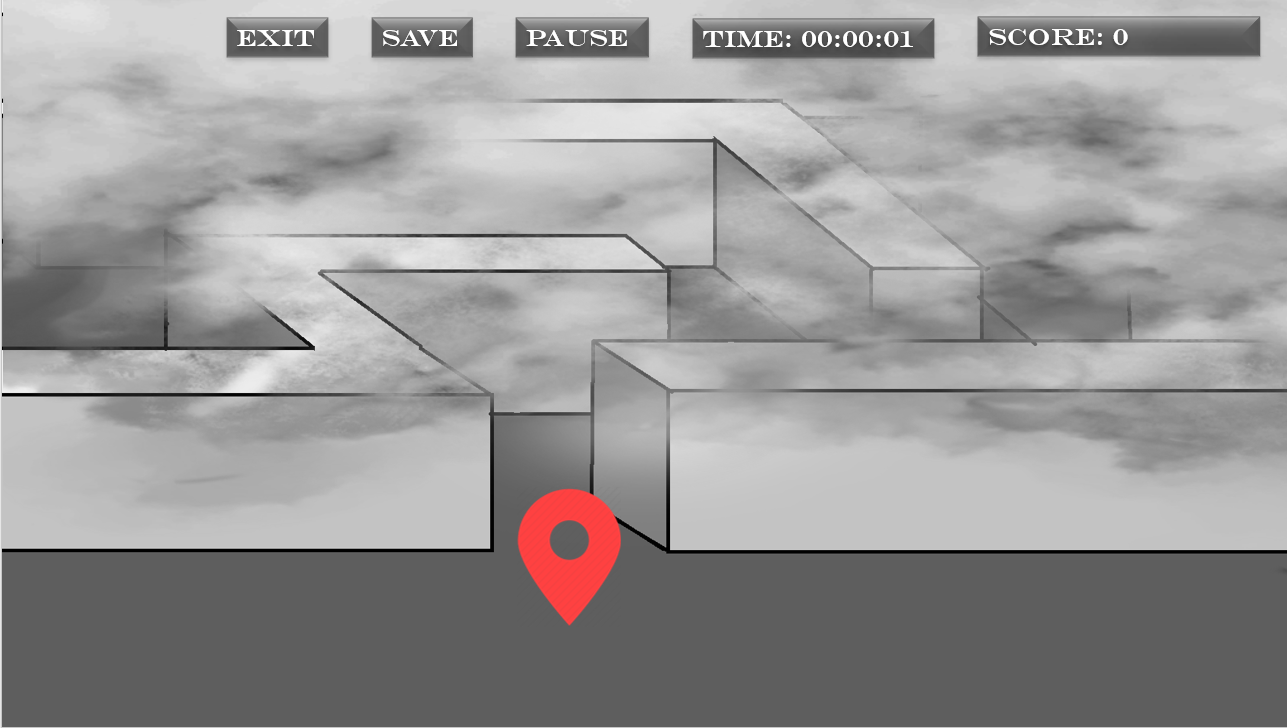
\includegraphics[height=150px, width=250px]{interface/Interface-BeginMaze.png}
\caption{This is the screen where the "New Button" transports the user}
\label{Start of Maze}
\end{figure}
\begin{figure}[ht!]
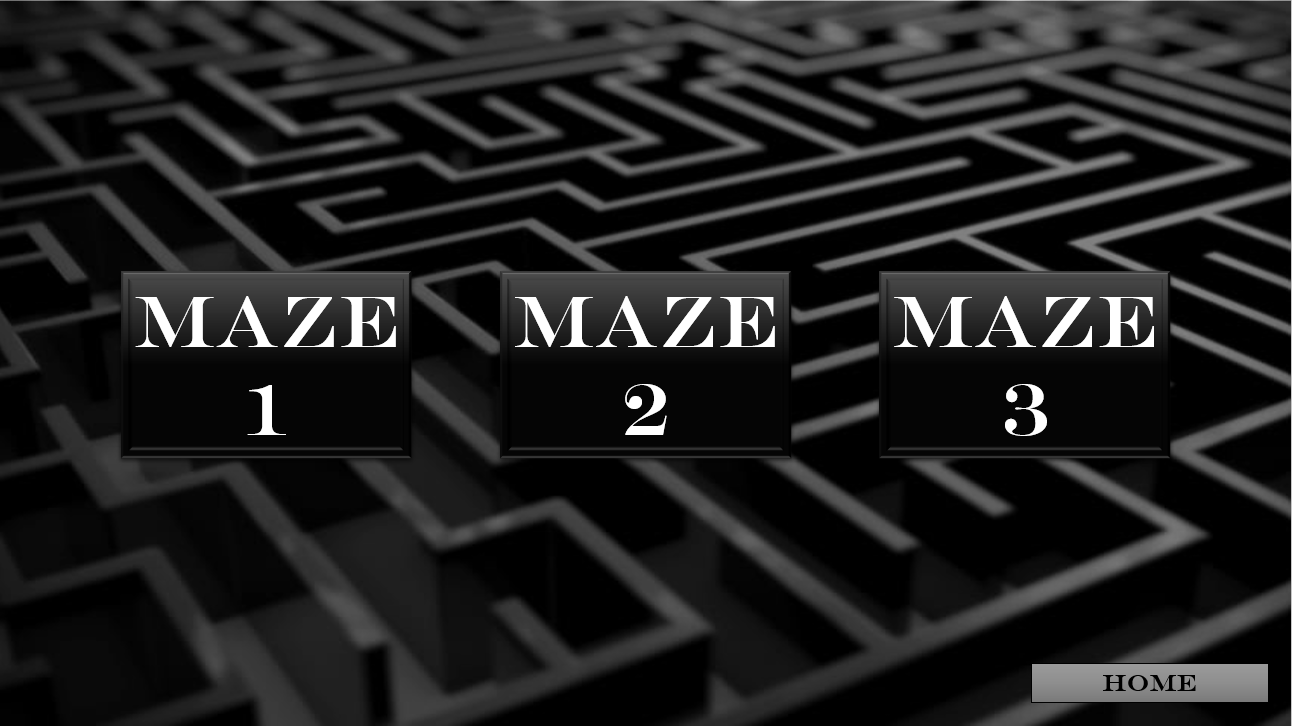
\includegraphics[height=150px, width=250px]{interface/Interface-Load.png}
\caption{This is the Load Screen that will appear after they select the button "Load Game"}
\label{Load Screen}
\end{figure}
\begin{figure}[ht!]
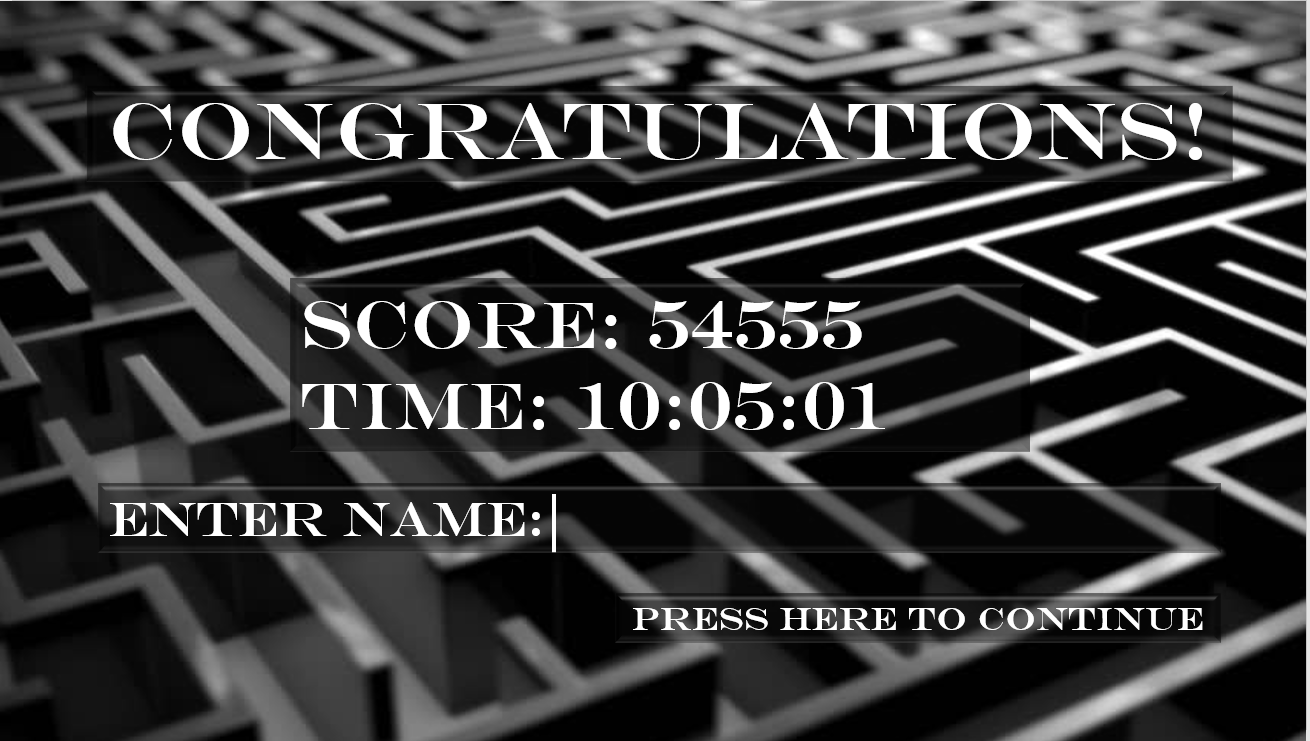
\includegraphics[height=150px, width=250px]{interface/Interface-Finish.png}
\caption{This is the screen that will be shown after the Maze game has finished}
\label{Finish Screen}
\end{figure}
\begin{figure}[ht!]
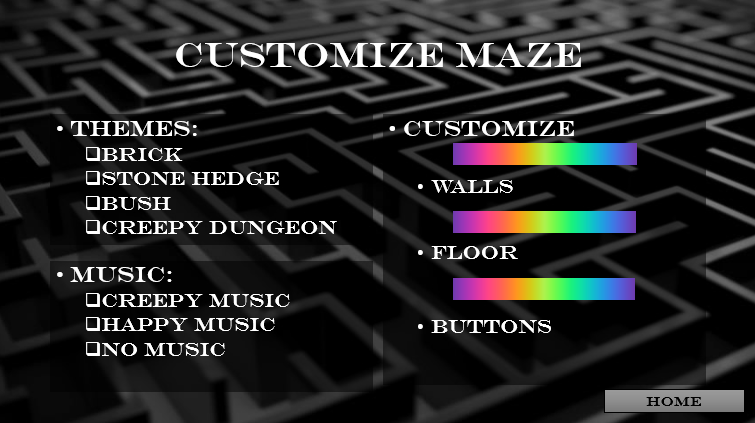
\includegraphics[height=150px, width=250px]{interface/Interface-Customize.png}
\caption{This is the Customize Menu}
\label{Customize Menu}
\end{figure}
\begin{figure}[ht!]
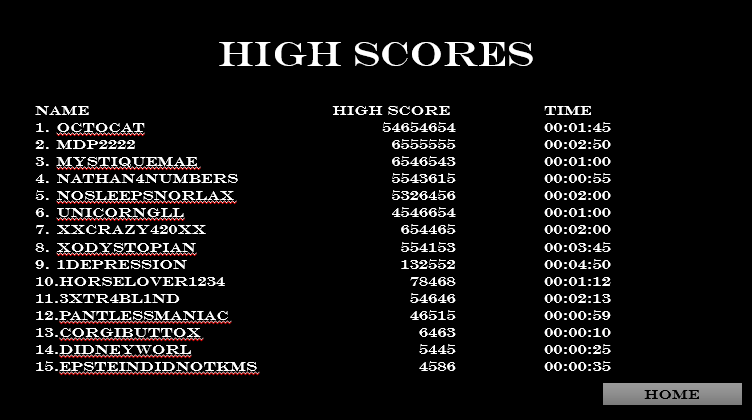
\includegraphics[height=150px, width=250px]{interface/Interface-HighScores.png}
\caption{This is the High Score Screen}
\label{High Scores}
\end{figure}
\begin{figure}[ht!]
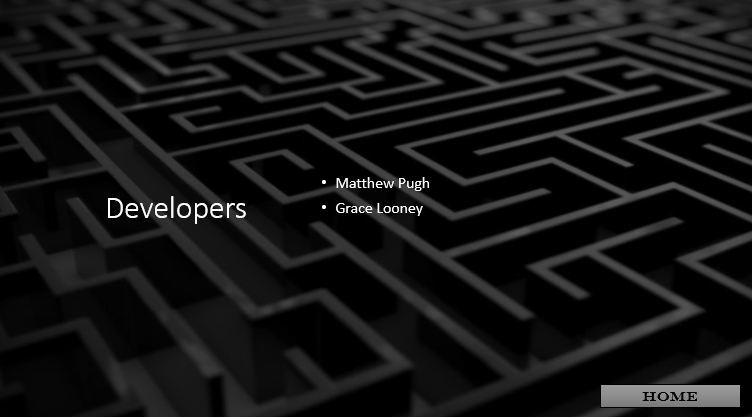
\includegraphics[height=150px, width=250px]{interface/Interface-Credits.png}
\caption{This is the Credits}
\label{Credits}
\end{figure}
\clearpage
\section{Project Timeline}

Maze Game Timeline: (refer to Table 2 for a more detailed schedule)
\begin{enumerate}
\item Requirements: January 20 - February 27
\item Design: February 28 – March 31
\item Implementation: April 1 – April 20
\item Verification: April 21 – April 26
\item Maintenance: April 26 - onward
\end{enumerate}
Explanation: 
\begin{itemize} 
\item Requirements
\begin{itemize}
\item Teams formed. Began planning what we wanted the game to do and look like. Decided what features we need/want to implement.
\end{itemize}
\item Design
\begin{itemize}
\item Planned out the programming structure of the maze game. Selected the Singleton and Observer design patterns to use in implementation of the game.
\end{itemize}
\item Implementation
\begin{itemize}
\item Full scale implementation of designs.
\begin{enumerate}
\item April 1 – April 7: Begin implementation of the main menu as well as the mazes themselves. Focus on completing the new game and load game options. If new game and load game are completed, begin implementing the high score page and settings menu.
\item April 8 – April 14: Continue implementation of the mazes and finish implementing the high score page and settings menu if they are not yet complete.
\item April 15 – April 20: Finish implementation of the mazes. Begin working on stretch goals (timer, music, secret buttons, hidden objects) if enough work is completed on the mazes.
\end{enumerate}
\end{itemize}
\item Verification
\begin{itemize}
\item Maze should be completed at this stage. Prepare for the final presentation on April 26.
\end{itemize}
\item Maintenance
\begin{itemize}
\item Review goals that were and were not accomplished. Discuss new features that may be implemented in the future.
\end{itemize}
\end{itemize} 

\begin{table}
\centering
\begin{tabular}{|l|c|c|c|c|}
\hline
 Activity & Start & End & Notes & Priority \\
\hline \hline
Requirements: \\
\hline \hline
Team Formed & 1/9/2020 & 1/11/2020 & A team of two exists and they tolerate each other & 1\\
Project Idea & 1/10/2020 & 1/15/2020 & Both members agree upon an idea & 1\\
Purpose & 1/21/2020 & 1/15/2020 & Both members agree upon the purpose of the project & 1\\
Features & 1/21/2020 & 1/15/2020 & Both members agree upon an what features to include& 1\\
Use Cases & 2/11/2020 & 1/15/2020 & The use cases are listed in the latex file & 1\\
Non-functional and functional & 2/11/2020 & 1/15/2020 & The requirements are listed in the latex file & 2\\
Interface Mockup & 2/11/2020 & 2/21/2020 & The mockup slides are added to the Latex file & 2\\
\hline \hline
Design: \\
\hline \hline 
Timeline & 2/26/2020 & 2/27/2020 & The timeline is added to the latex file & 2\\
UML Outline & 2/28/2020 & 3/31/2020 & The outline is added to the latex file & 2\\
Researched Design Patterns& 2/27/2020& 3/31/2020 & The team reasearches possible design patterns to implement & 3\\
Researched Implementation Ideas & 2/29/2020& 3/31/2020 & The team reasearches possible ways to implement project & 3\\
Updated Latex File& 3/31/2020 & 3/31/2020 & The team updates the Latex file with the changes&2\\
\hline \hline
Implementation: \\
\hline \hline 
Main Menu &4/1/2020& 4/8/2020& Main menu implementation should be complete& 2\\
Maze&4/1/2020 & 4/14/2020 & Maze implementation should be complete& 1\\
High Score& 4/8/2020&4/16/2020& High score implementation should be complete& 2\\
Settings&4/1/2020& 4/14/2020& settings menu implementation should be complete& 2\\
Stretch Goals& 4/15/2020&4/21/2020& Stretch goals should implementation should be attempted & 3\\
\hline \hline
Verification: \\
\hline \hline 
Testing & 4/15/2020&4/20/2020&Test project&1\\
Preparation for Presentation & 4/20/2020&4/20/2020& Prepare&1\\
\hline
\end{tabular}
\caption{Timeline Table}
\label{tab:timeline}
\end{table}
\clearpage
\section{Project Structure}
At first, this will be a little empty (it will need to be filled in by the time you turn in your final report).  This is your chance to discuss all of your design decisions (consider this the README's big brother).

\subsection{UML Outline}
\begin{figure}[ht!]
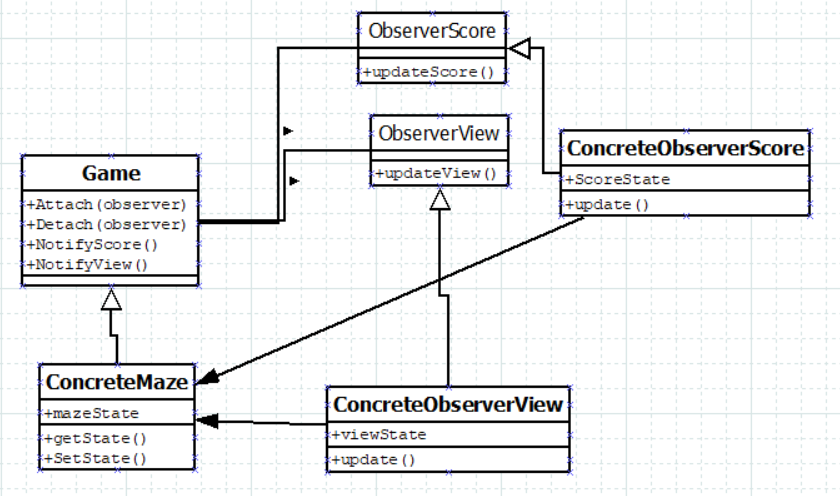
\includegraphics[scale=.5]{patterns/Observer.png}
\caption{How we will update the GUI}
\label{Game play}
\end{figure}
\begin{figure}[ht!]
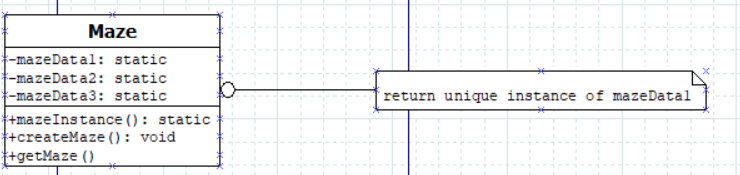
\includegraphics[scale=.5]{patterns/Singleton.png}
\caption{How we will handle the three instances of the maze}
\label{Maze instance}
\end{figure}
\clearpage
\subsection{Design Patterns Used}
\begin{enumerate}
\item Singleton
\item Factory
\end{enumerate}


\section{Results}
This section will start out a little vague, but it should grow as your project evolves.  With each deliverable you hand in, give me a final summary of where your project stands.  By the end, this should be a reflective section discussing how many of your original goals you managed to attain/how many desired use cases you implemented/how many extra features you added.

\subsection{Future Work}
Where are you going next with your project?
For early deliverables, what are your next steps?  (HINT: you will typically want to look back at your timeline and evaluate: did you meet your expected goals?  Are you ahead of schedule?  Did you decide to shift gears and implement a new feature?)
By the end, what do you plan on doing with this project?  Will you try to sell it?  Set it on fire?  Link to it on your resume and forget it exists?




\begin{thebibliography}{1}

\bibitem{IEEEhowto:kopka}
H.~Kopka and P.~W. Daly, \emph{A Guide to \LaTeX}, 3rd~ed.\hskip 1em plus
  0.5em minus 0.4em\relax Harlow, England: Addison-Wesley, 1999.
\bibitem{Pullen}
Walter Pullen. \emph{Think Labyrinth},(2012).
\end{thebibliography}



\begin{IEEEbiography}{Michael Shell}
Biography text here.
\end{IEEEbiography}

% if you will not have a photo at all:
\begin{IEEEbiographynophoto}{John Doe}
Biography text here.
\end{IEEEbiographynophoto}

% insert where needed to balance the two columns on the last page with
% biographies
%\newpage

\begin{IEEEbiographynophoto}{Jane Doe}
Biography text here.
\end{IEEEbiographynophoto}





% that's all folks
\end{document}
